%\documentclass[
  bibliography=totoc,     % Literatur im Inhaltsverzeichnis
  captions=tableheading,  % Tabellenüberschriften
  titlepage=firstiscover, % Titelseite ist Deckblatt
]{scrartcl}

% Paket float verbessern
\usepackage{scrhack}

% Warnung, falls nochmal kompiliert werden muss
\usepackage[aux]{rerunfilecheck}

% unverzichtbare Mathe-Befehle
\usepackage{amsmath}
% viele Mathe-Symbole
\usepackage{amssymb}
% Erweiterungen für amsmath
\usepackage{mathtools}

% Fonteinstellungen
\usepackage{fontspec}
% Latin Modern Fonts werden automatisch geladen
% Alternativ zum Beispiel:
%\setromanfont{Libertinus Serif}
%\setsansfont{Libertinus Sans}
%\setmonofont{Libertinus Mono}

% Wenn man andere Schriftarten gesetzt hat,
% sollte man das Seiten-Layout neu berechnen lassen
\recalctypearea{}

% deutsche Spracheinstellungen
\usepackage[ngerman]{babel}


\usepackage[
  math-style=ISO,    % ┐
  bold-style=ISO,    % │
  sans-style=italic, % │ ISO-Standard folgen
  nabla=upright,     % │
  partial=upright,   % │
  mathrm=sym,        % ┘
  warnings-off={           % ┐
    mathtools-colon,       % │ unnötige Warnungen ausschalten
    mathtools-overbracket, % │
  },                       % ┘
]{unicode-math}

% traditionelle Fonts für Mathematik
\setmathfont{Latin Modern Math}
% Alternativ zum Beispiel:
%\setmathfont{Libertinus Math}

\setmathfont{XITS Math}[range={scr, bfscr}]
\setmathfont{XITS Math}[range={cal, bfcal}, StylisticSet=1]

% Zahlen und Einheiten
\usepackage[
  locale=DE,                   % deutsche Einstellungen
  separate-uncertainty=true,   % immer Unsicherheit mit \pm
  per-mode=symbol-or-fraction, % / in inline math, fraction in display math
]{siunitx}

% chemische Formeln
\usepackage[
  version=4,
  math-greek=default, % ┐ mit unicode-math zusammenarbeiten
  text-greek=default, % ┘
]{mhchem}

% richtige Anführungszeichen
\usepackage[autostyle]{csquotes}

% schöne Brüche im Text
\usepackage{xfrac}

% Standardplatzierung für Floats einstellen
\usepackage{float}
\floatplacement{figure}{htbp}
\floatplacement{table}{htbp}

% Floats innerhalb einer Section halten
\usepackage[
  section, % Floats innerhalb der Section halten
  below,   % unterhalb der Section aber auf der selben Seite ist ok
]{placeins}

% Seite drehen für breite Tabellen: landscape Umgebung
\usepackage{pdflscape}

% Captions schöner machen.
\usepackage[
  labelfont=bf,        % Tabelle x: Abbildung y: ist jetzt fett
  font=small,          % Schrift etwas kleiner als Dokument
  width=0.9\textwidth, % maximale Breite einer Caption schmaler
]{caption}
% subfigure, subtable, subref
\usepackage{subcaption}

% Grafiken können eingebunden werden
\usepackage{graphicx}

% schöne Tabellen
\usepackage{tabularray}
\UseTblrLibrary{booktabs, siunitx}

% Verbesserungen am Schriftbild
\usepackage{microtype}

% Literaturverzeichnis
\usepackage[
  backend=biber,
]{biblatex}
% Quellendatenbank
\addbibresource{lit.bib}
\addbibresource{programme.bib}

% Hyperlinks im Dokument
\usepackage[
  german,
  unicode,        % Unicode in PDF-Attributen erlauben
  pdfusetitle,    % Titel, Autoren und Datum als PDF-Attribute
  pdfcreator={},  % ┐ PDF-Attribute säubern
  pdfproducer={}, % ┘
]{hyperref}
% erweiterte Bookmarks im PDF
\usepackage{bookmark}

% Trennung von Wörtern mit Strichen
\usepackage[shortcuts]{extdash}

\author{%
  Vincent Wirsdörfer\\%
  \href{mailto:vincent.wirsdoerfer@udo.edu}{authorA@udo.edu}%
  \and%
  Joris Daus\\%
  \href{mailto:joris.daus@udo.edu}{authorB@udo.edu}%
}
\publishers{TU Dortmund – Fakultät Physik}


%\begin{document}
%\section{Versuchsaufbau}

\section{Versuchsdurchführung}

Der allgemeine Versuchsaufbau wird in der unten stehenden Abbildung visualisiert.

\begin{figure}
    \centering
    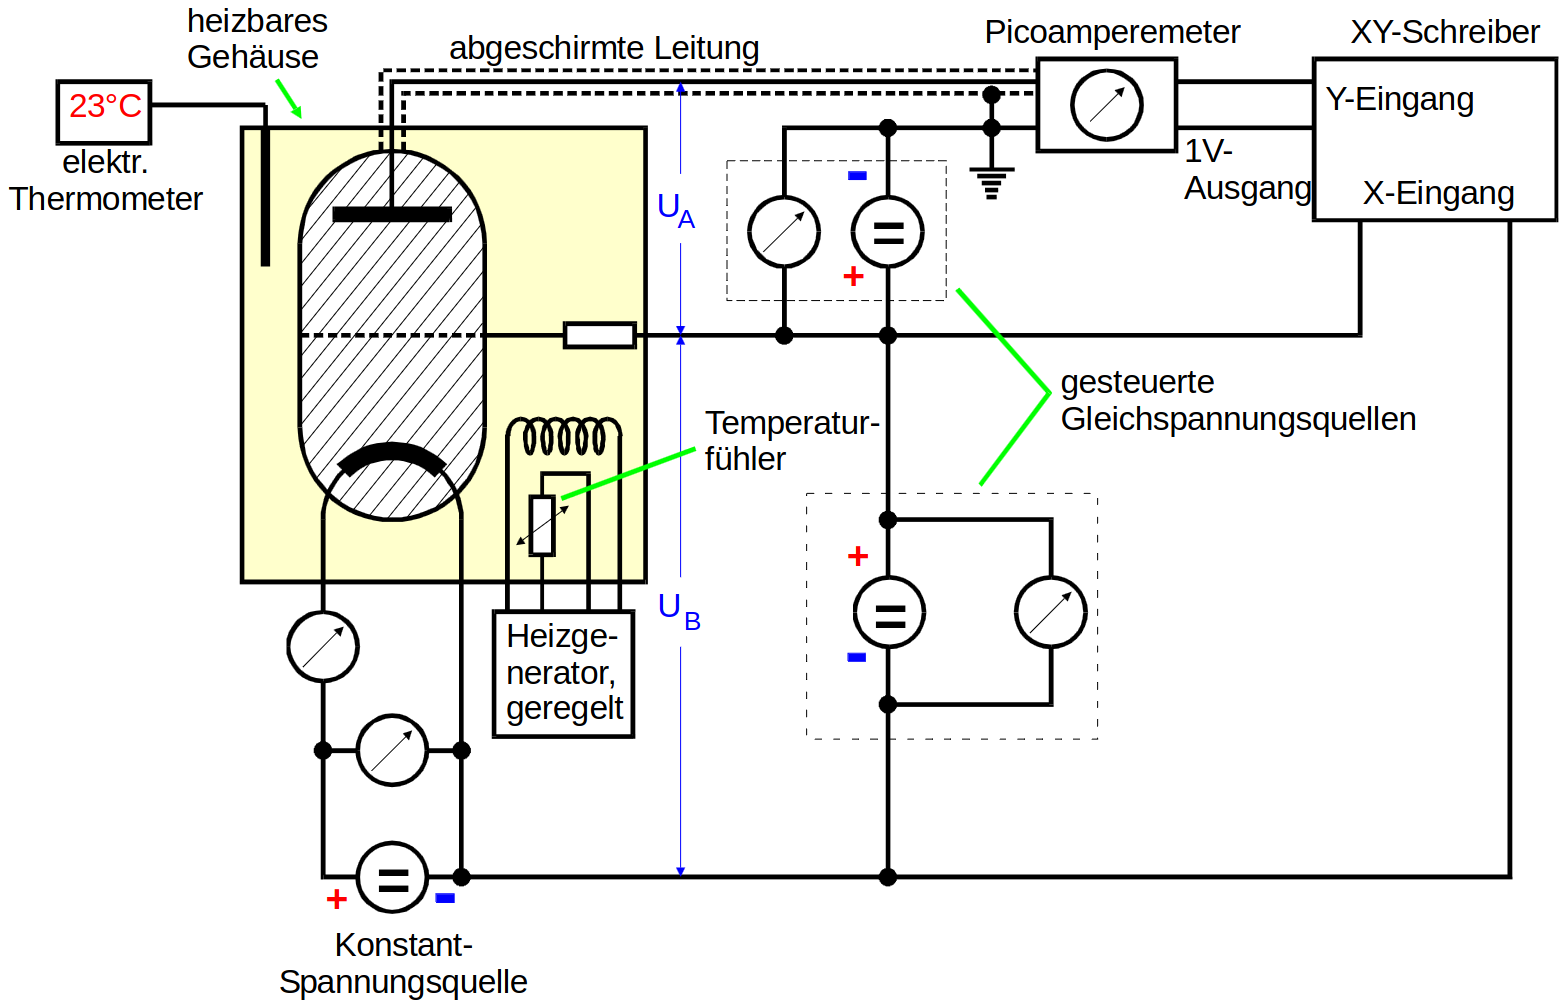
\includegraphics[height=6cm]{content/Aufbau.png}
    \caption{Versuchsaufbau des Franck-Hertz-Experiments\cite{Versuchsanleitung_v601}.}
    \label{fig:Aufbau}
\end{figure}

\noindent Zwangsweise wurden die grundlegenden Elemente des Franck-Hertz-Versuchs in der Theorie \ref{sec:Theorie} nahgelegt. Hauptbestandteil ist dabei 
das heizbare Gehäuse, welches die Quecksilber-Kammer sowie alle notwendigen Kathoden und Elektroden enthält. Der Großteil der quantenphysikalischen Entdeckung 
des Experiments wird somit bereits abgedeckt. Über ein elektrisches Thermometer kann die Temperatur des Gehäuses. Ein weiterer Bestandteil des Aufbaus ist 
das Picoamperemeter, welches den Auffängerstrom $I_\text{A}$ misst und an den XY-Schreiber weitergibt. Die detektierten Elektronen können somit auf Papier 
gebracht werden.\\

\noindent Zu Beginn des Versuchs werden alle Ein- und Ausgänge der relevanten Geräte verkabelt und von der Betreuerin überprüfen lassen. Im ersten Teil des Versuchs wird 
die integrale Energieverteilung der Elektronen untersucht. Hierzu wird bei einer konstanten Beschleunigungsspannung von $U_\text{B} = \qty{9}{\volt}$ der 
Auffängerstrom $I_\text{A}$ als Funktion der Bremsspannung $U_\text{A}$ gemessen. Das Intervall der Bremsspannung beträgt dabei [$\qty{0}{\volt};\qty{10}{\volt}$]. 
Hiebei wird je eine Messung bei Zimmertemperatur ($T \approx \qty{298.15}{\kelvin}$) und eine Messung bei einer erhöhten Temperatur von $T = \qty{414.55}{\kelvin}$
durchgeführt.\\

\noindent Im Anschluss wird die Franck-Hertz-Kurve für verschiedenen Temperaturen aufgenommen. Dementsprechend wird die Versuchsapparatur erneut verkabelt, sodass 
nun der Auffängerstrom als Funktion der Beschleunigunsspannung in einem Intervall [$\qty{0}{\volt};\qty{60}{\volt}$] gemessen werden kann. Die jetzt kosntante 
Bremsspannung hat den den Wert $U_\text{A} = \qty{1}{\volt}$. Die Franck-Hertz-Kurven werden bei den folgenden Temperaturen aufgezeichnet:

\begin{align*}
    T1 &= \qty{438.15}{\kelvin} \\ 
    T2 &= \qty{447.15}{\kelvin} \\  
    T3 &= \qty{459.15}{\kelvin} \\  
\end{align*}


%\section{Messwerte}

%\end{document}

